% -*- latex -*-
% c4.tex
% LabSK 12.04.2022

% Wymagane pola (komentarz):
% Dawid Chmielewski				% Imię Nazwisko
% Praca w linii poleceń		% Temat ćwiczenia

\documentclass[a4paper,11pt]{article}

\usepackage[T1]{polski}
\usepackage[utf8]{inputenc}  			% Kodowanie pliku
\usepackage{pdfpages}

\hoffset=-3.0cm                         % Mniejszy lewy margines
\textwidth=18cm                         % szerzej
\evensidemargin=0pt

\voffset=-3cm                           % Mniejszy górny margines
\textheight=27cm                        % szerzej wzdłuż

\setlength{\parindent}{0pt}             % Paragraf od początku linii
\setlength{\parskip}{\medskipamount}    % Odstęp pomiędzy paragrafami
\raggedbottom                           % bez rozciągania strony

% Dodatkowe komendy
\newcommand\BS{\char`\\}                % \BS == back-slash
\newcommand\TY{\raise.17ex\hbox{$\scriptstyle\mathtt{\sim}$}}   % \TY == większa tylda w \tt

\thispagestyle{empty}			        % bez numeracji stron
\usepackage{enumerate}

\begin{document}
\title{ Sieci komputerowe - sprawozdanie z ćwiczenia 4. }
\author{ Dawid Chmielewski, numer indeksu: 311188 }
\date{3 maja 2022}

\maketitle{Temat ćwiczenia: Serwis DHCP.}

\section{Ogólny cel ćwiczenia}

Tematem ćwiczenia był pełen serwis DHCP wraz z jego analizą.

\section{Skrypt PowerShell zdejmujący nadanie adresu IPv4 przez DHCP}

Algorytm działania skryptu (w kolejności działania):

1. Włączenie programu tshark, nastawienie programu tshark na pięć pakietów przychodzących na interfejsie Wi-Fi,

2. Zdjęcie adresu DHCP (po pięciu sekundach od uruchomienia skryptu) poleceniem {\tt ipconfig /release},

3. Odczekanie pięciu sekund,

4. Odnowienie DHCP poleceniem {\tt ipconfig /renew}.

Budowa skryptu:


{\tt
\begin{verbatim}
    Start-Job -Name labsk4 -ScriptBlock {
	    Start-Sleep -s 5
	    ipconfig /release
	    Start-Sleep -s 5
	    ipconfig /renew
    }
    tshark -i "Wi-Fi" -f "port 67 or port 68" -c5 -F pcap -w dhcp.pcap
\end{verbatim}
}


\section{Minimalny schemat sieci}

Na następnej strone prezentuję schemat sieci narysowany przeze mnie w draw.io.

\pagebreak
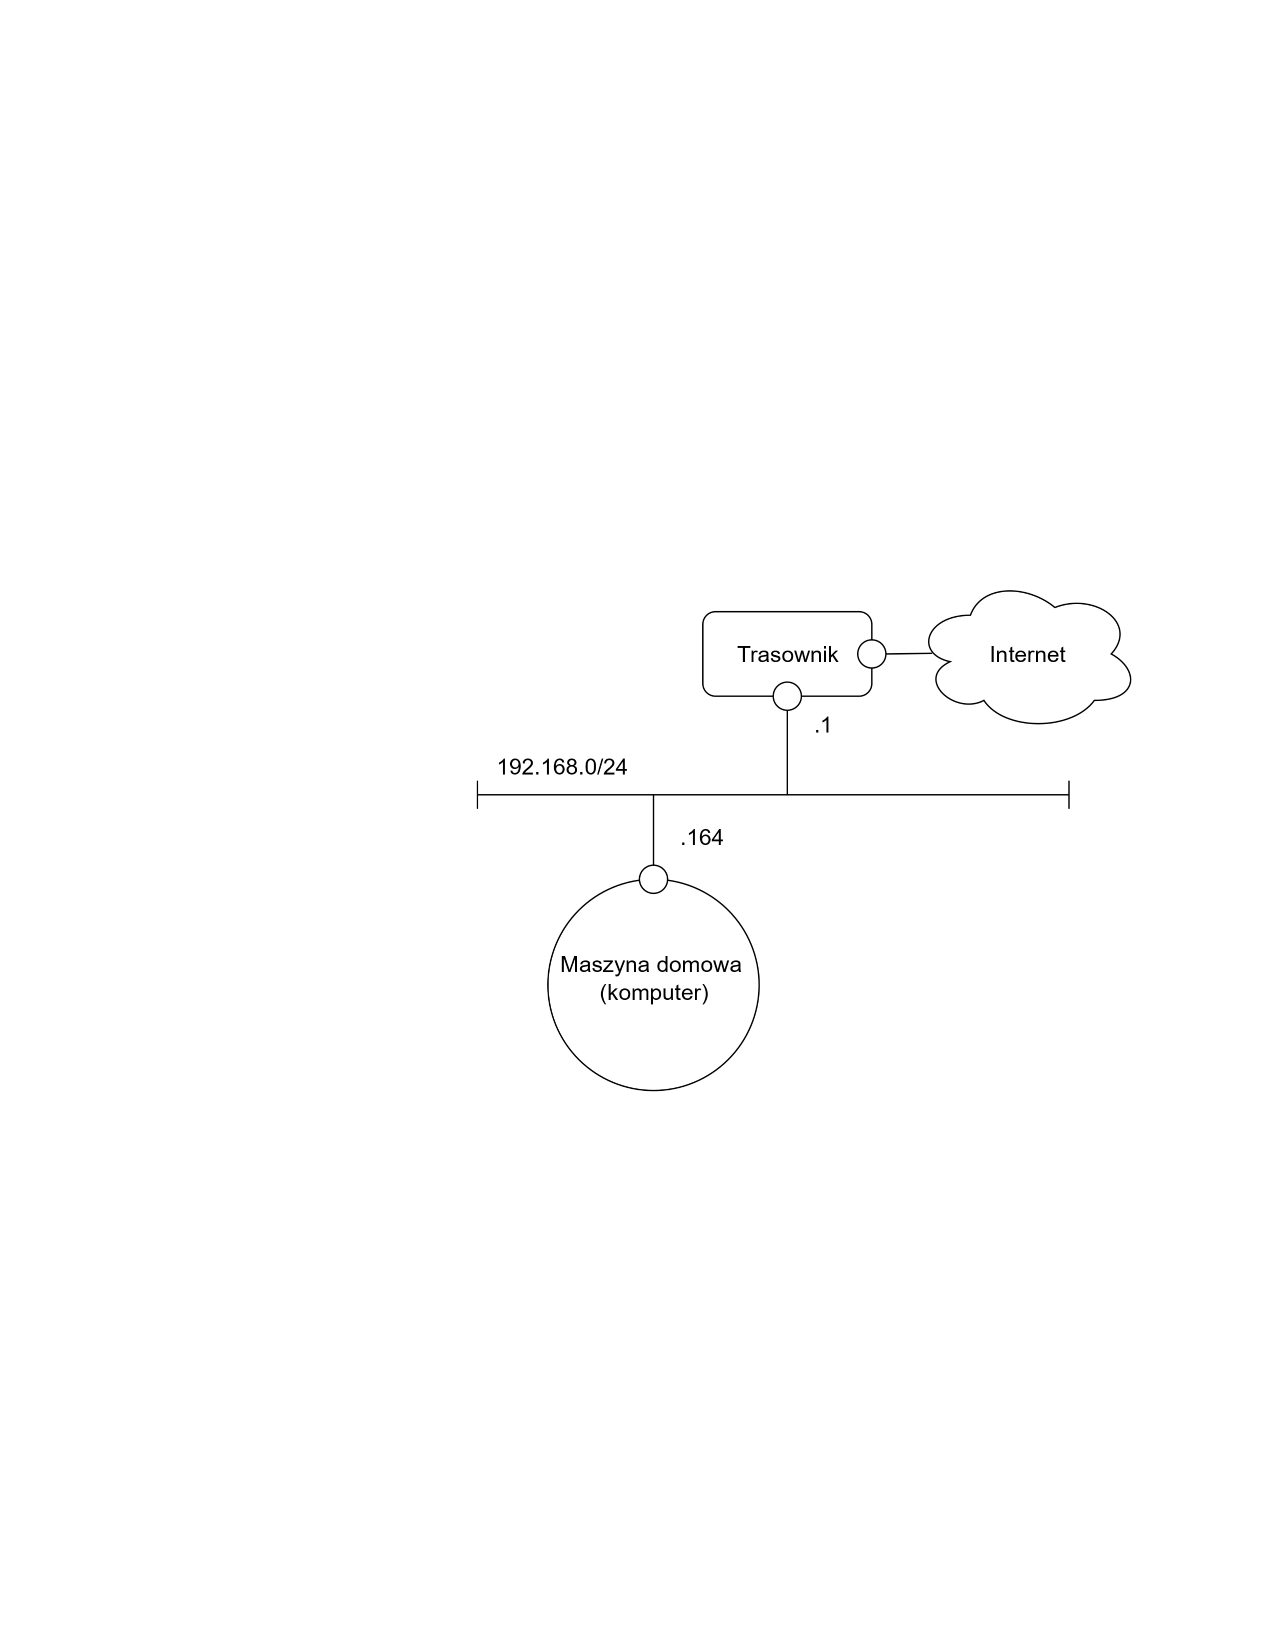
\includepdf[pages=-]{diagram_c4.pdf}

\section{Analiza informacji przesłanych przez DHCP}

Podgląd pliku dhcp.pcap utworzonego w wyniku działania mojego skryptu:

{\tt
\begin{verbatim}
    1	0.000000	192.168.0.164	192.168.0.1	DHCP	342	DHCP Release  - Transaction ID 0x3367c9eb
    2	5.115133	0.0.0.0	255.255.255.255	DHCP	344	DHCP Discover - Transaction ID 0xa9bd3db8
    3	5.154147	192.168.0.1	192.168.0.164	DHCP	590	DHCP Offer    - Transaction ID 0xa9bd3db8
    4	5.154786	0.0.0.0	255.255.255.255	DHCP	370	DHCP Request  - Transaction ID 0xa9bd3db8
    5	5.275099	192.168.0.1	192.168.0.164	DHCP	590	DHCP ACK      - Transaction ID 0xa9bd3db8
\end{verbatim}
}

Każda linia w pliku zawiera następujące informacje: numer pakietu w kolejności, czas od wpłynięcia pierwszego pakietu (w sekundach), adres IP źródła i celu, rodzaj protokołu (tutaj: wszystkie pakiety mają rodzaj DHCP), długość w bajtach, nazwa komunikatu oraz ID transakcji.

\begin{itemize}
    \item Release- komunikat wysłany przez moją maszynę przy użyciu {\tt ipconfig /release}- odrzucenie aktualnie posiadanego adresu IP,
    \item Discover- wyszukiwanie serwera DHCP przez klienta, adres 0.0.0.0 świadczy o braku adresu IP klienta (został zdjęty), zaś adres 255.255.255.255- adres rozgłoszeniowy (klient szuka serwera, wysyłając komunikat do wszystkich),
    \item Offer- odpowiedź serwera oferująca klientowi dzierżawę adresu IP,
    \item Request- akceptacja dzierżawy adresu IP przez klienta,
    \item ACK- potwierdzenie przez serwera użycia adresu żądanego przez klienta.
\end{itemize}

\section{Stan konfigurowanego interfejsu przed i po DHCP}

Poniżej prezentuję stan konfigurowanego interfejsu (Wireless LAN adapter Wi-Fi) przed i po DHCP. Jak widać został nadany adres IPv4.

Przed DHCP:

{\tt
\begin{verbatim}
Wireless LAN adapter Wi-Fi:

   Connection-specific DNS Suffix  . :
   IPv6 Address. . . . . . . . . . . : 2a02:a312:340:8a00:9017:d092:9ed0:641f
   Temporary IPv6 Address. . . . . . : 2a02:a312:340:8a00:819c:8812:dafc:2c4
   Link-local IPv6 Address . . . . . : fe80::9017:d092:9ed0:641f%9
   Default Gateway . . . . . . . . . : fe80::de53:7cff:feb7:b75d%9
   
\end{verbatim}
}

po DHCP:

{\tt
\begin{verbatim}
Wireless LAN adapter Wi-Fi:

   Connection-specific DNS Suffix  . : home
   IPv6 Address. . . . . . . . . . . : 2a02:a312:340:8a00:9017:d092:9ed0:641f
   Temporary IPv6 Address. . . . . . : 2a02:a312:340:8a00:819c:8812:dafc:2c4
   Link-local IPv6 Address . . . . . : fe80::9017:d092:9ed0:641f%9
   IPv4 Address. . . . . . . . . . . : 192.168.0.164
   Subnet Mask . . . . . . . . . . . : 255.255.255.0
   Default Gateway . . . . . . . . . : fe80::de53:7cff:feb7:b75d%9
                                       192.168.0.1
   
\end{verbatim}
}

\section{Zrzut ekranu konfiguracji DHCP}

Moim dostawcą internetu domowego jest UPC. Na następnej stronie prezentuję zrzut ekranu konfiguracji DHCP.


\begin{figure}[h!]
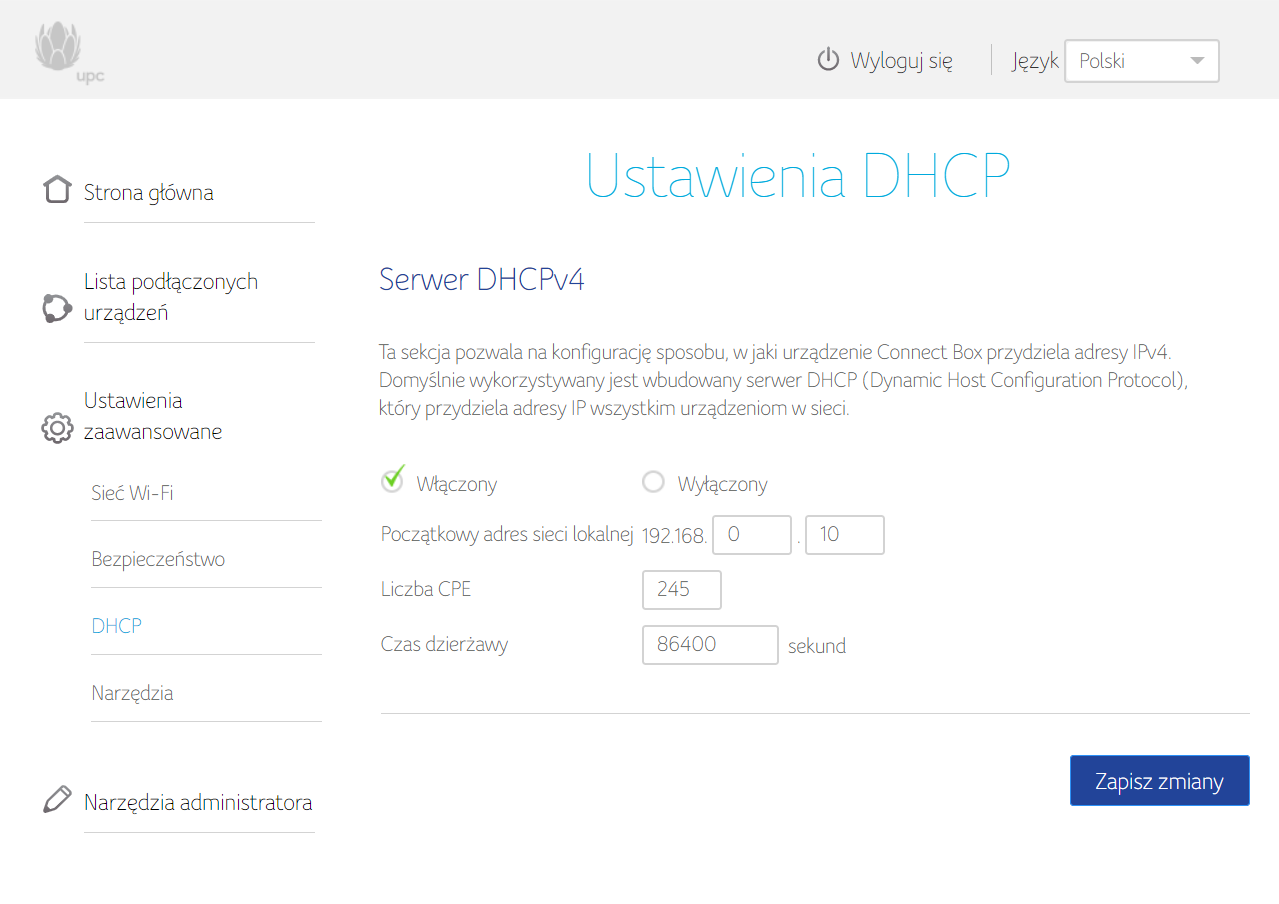
\includegraphics[scale=0.7]{ekran-konfiguracji}
\end{figure}

\end{document}